\newpage
\chapter{Smart Grid: architettura, componenti ed evoluzione}

\section{Introduzione alle Smart Grid}



Una Smart Grid - Rete Intelligente - è l'evoluzione della tradizionale rete elettrica. Si basa su componenti avanzati di \textbf{rilevamento}, \textbf{comunicazione} e \textbf{decisione} per ottenere una trasmissione e distribuzione di energia \textbf{sicura}, \textbf{efficiente} e \textbf{resiliente}. \cite{en15186799}


L'aumento di anno in anno di fonti rinnovabili ha portato ad una crescita significativa della generazione di energia distribuita, ovvero la produzione di energia tramite piccoli impianti connessi alla rete di distribuzione elettrica. In questo contesto di flussi non più monodirezionali, bensì bidirezionali, l'utilizzo di Smart Grid possono essere di grande aiuto per le aziende di Trasmissione e Distribuzione dell'energia elettrica. \cite{Enel}


\begin{figure}[h!]
    \centering
    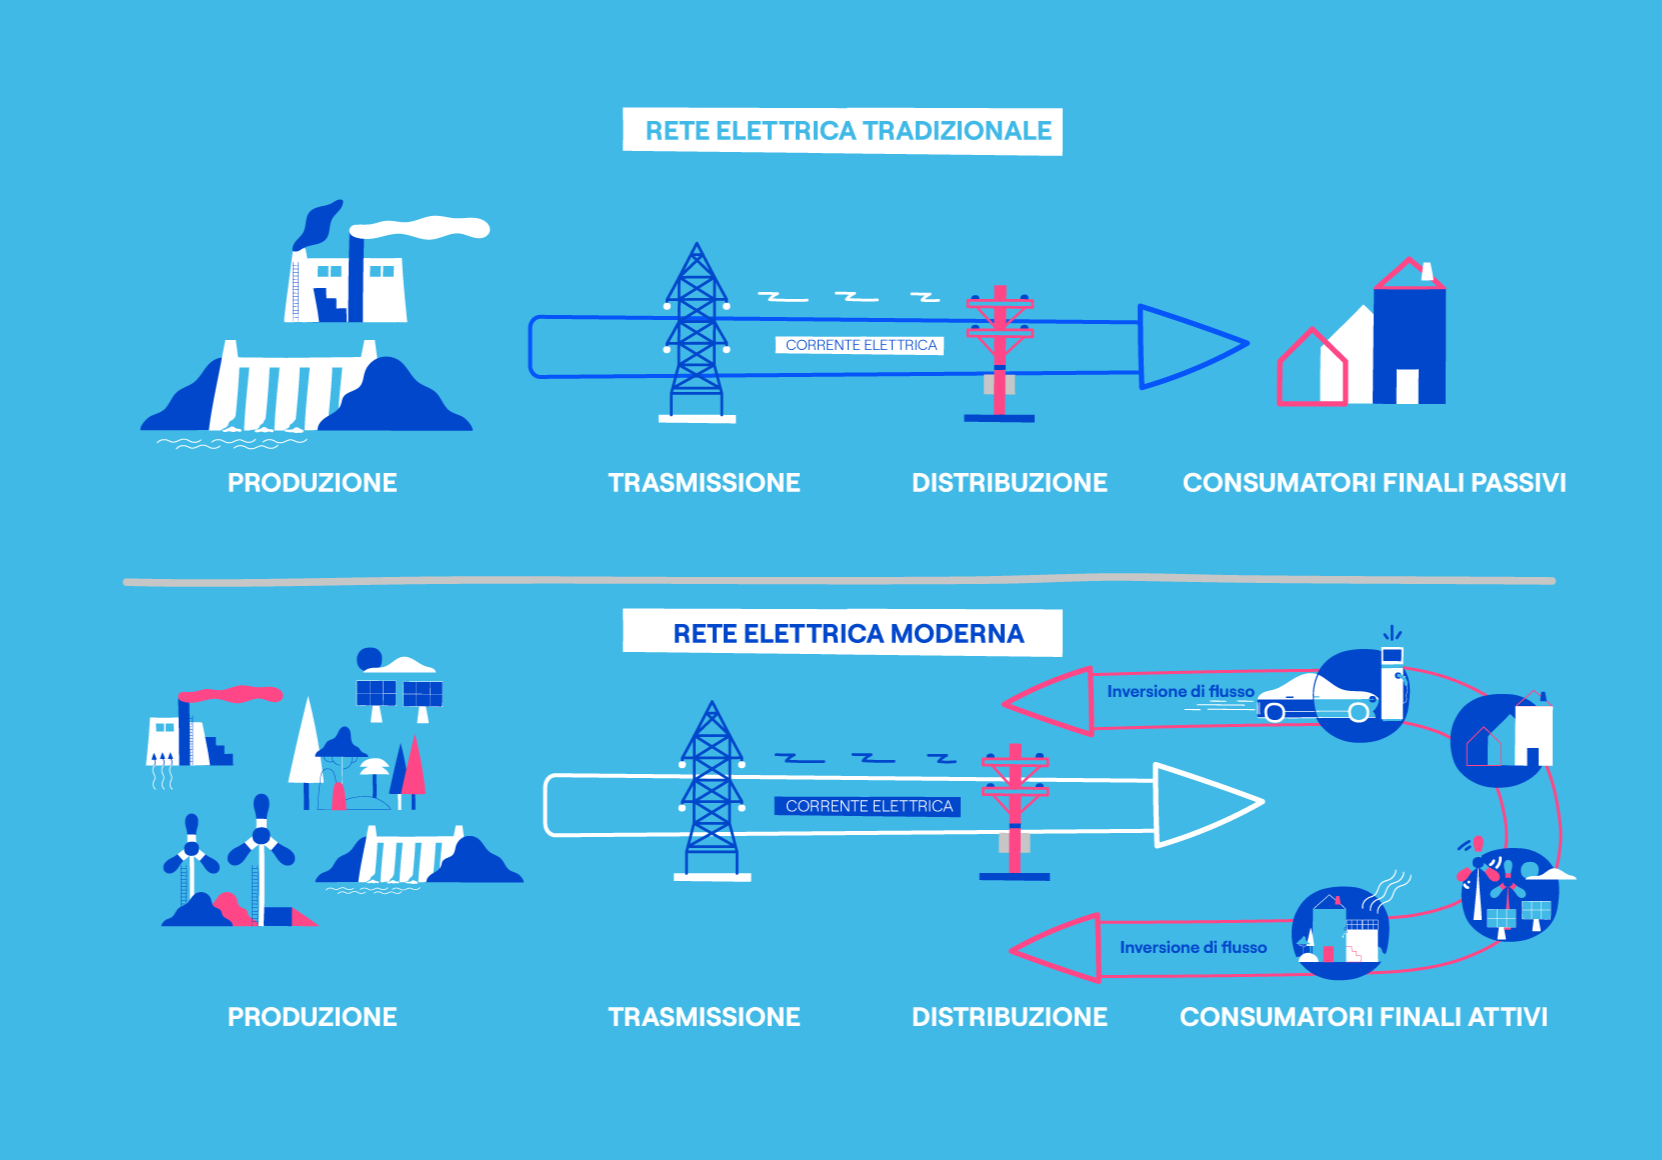
\includegraphics[width=0.8\linewidth]{img/Smart-Grid-EDistribuzione2.png}
    \caption{Confronto rete tradizionale e rete intelligente}
    \label{fig:TraditionalGridVSSmartrGrid}
\end{figure}


Come si può vedere anche nella Figura \ref{fig:TraditionalGridVSSmartrGrid} la Smart Grid si compone di 4 parti fondamentali: la \textit{Produzione}, la 
\textit{Trasmissione}, la \textit{Distribuzione} e infine le \textit{Utenze}.

% \begin{center}
%     \textit{Produzione} - \textit{Trasmissione} - \textit{Distribuzione} - \textit{Utenze}
% \end{center}

\newpage
\subsection{Produzione}

La produzione di elettricità, sia nel sistema tradizionale sia con l'utilizzo delle Smart Grid, avviene attraverso un mix energetico di Fonti Energetiche NON Rinnovabili (\textbf{non FER}) e Fonti Energetiche Rinnovabili (\textbf{FER}).

In Italia la produzione, e non l'importazione, di energia elettrica avviene sfruttando varie fonti tra cui le non FER, con circa il 54\%, e il restante 46\% proviene invece dalle fonti FER Tabella \ref{tab:GSE-mix-nazionale-2023}.

In particolare come riportato nel "Rapporto Mensile sul Sistema Elettrico 2024" redatto da Terna \cite{TernaRapporto2024} si mostra che l'assorbimento totale, la somma di produzione più importazioni di energia elettrica, nel periodo Gen-Dic 2024 è stata di $312\ TWh$, di cui FER \footnote{Produzione da FER = Idrico + Biomasse + Geotermico + Eolico + Fotovoltaico} $129\ TWh\ (49\%)$, non FER $132\ TWh\ (51\%)$ e importazioni $51\ TWh$.






% \begin{table}
%     \renewcommand{\arraystretch}{2}
%     \centering
%     \begin{tabular}{c|c}
%         \multicolumn{2}{c}{\shortstack{Composizione del mix iniziale nazionale utilizzato per la produzione \\ dell'energia elettrica immessa nel sistema elettrico italiano nel 2023}}\\
%         \hline
%          Fonti primarie utilizzate	& \% \\
%          Fonti rinnovabili & 46 \\
%          Gas naturale& 43 \\
%          Carbone& 5 \\
%          Altre fonti & 5 \\
%          Prodotti petroliferi& 1 \\
%     \end{tabular}
%     \caption{Mix nazionale 2023}
%     \label{tab:GSE-mix-nazionale-2023}
% \end{table}

\begin{table}
    \renewcommand{\arraystretch}{2}
    \centering
    \begin{tabular}{c|c}
        % \multicolumn{2}{c}{\shortstack{}}\\
         % \multicolumn{2}{c}{Fonti primarie utilizzate \%} \\
         Fonti primarie utilizzate	& \% \\
         \hline
         Fonti rinnovabili & 46 \\
         Gas naturale& 43 \\
         Carbone& 5 \\
         Altre fonti & 5 \\
         Prodotti petroliferi& 1 \\
    \end{tabular}
    \caption{Composizione del mix iniziale nazionale immessa nel anno 2023 \cite{GSE}}
    \label{tab:GSE-mix-nazionale-2023}
\end{table}
